\documentclass[a4paper,11pt]{article}
\usepackage[utf8]{inputenc}
\usepackage[T1]{fontenc}
\usepackage{lmodern}
\usepackage{graphicx}
\usepackage{amsmath,amssymb}
\usepackage{hyperref}
\usepackage{float}
\usepackage{listings}
\usepackage{xcolor}
\usepackage{caption}
\usepackage{subcaption}

% Settings for code listings
\lstset{
  basicstyle=\ttfamily\small,
  keywordstyle=\color{blue},
  stringstyle=\color{red!60!black},
  commentstyle=\color{gray!70},
  frame=single,
  breaklines=true,
  numbers=left,
  numberstyle=\tiny,
  showstringspaces=false
}

\title{\textbf{Relazione Settimanale: Valutazione e Clustering di Risposte LLM}}%
\author{Team di Ricerca e Sviluppo ML}
\date{Settimana 21--27 Aprile 2025}

\begin{document}
\maketitle

\begin{abstract}
Questa relazione fornisce un'analisi approfondita delle attività svolte nella settimana corrente, finalizzate alla progettazione e implementazione di una pipeline di valutazione automatizzata di risposte generiche da modelli di linguaggio (LLM). In particolare, descriviamo:
\begin{itemize}
  \item il recupero e l'utilizzo di un modello di \emph{sequence classification} fine-tuned su Hugging Face per la classificazione di risposte non etichettate;
  \item la costruzione di rappresentazioni vettoriali bidimensionali e ad alta dimensionalità mediante estrazione di embedding da token speciali e metodi di riduzione dimensionale;
  \item l'applicazione dell'algoritmo di clustering K-Means per l'aggregazione e la valutazione delle risposte;
  \item miglioramenti introdotti su suggerimento del Prof. Ferretti, quali l'estensione del dataset e la raffinazione degli embedding;
  \item un confronto sperimentale con un modello BERT base non affinato per quantificare i benefici del fine tuning.
\end{itemize}
Il documento si conclude con una disamina dettagliata del codice Python sviluppato, suddiviso in blocchi funzionali, e con un rimando ai risultati quantitativi riportati nel file \texttt{Risultati\_Differenza\_BERT\_Tuned\_vs\_NonTuned.pdf}.
\end{abstract}

\section{Obiettivi e Metodologia}
L'obiettivo primario di questa settimana è stato implementare una pipeline in ambiente Colab che:
\begin{enumerate}
  \item carichi un modello LLM fine-tuned per compiti di classificazione di sequenze;
  \item generi vettori di features secondo due paradigmi: bidimensionale (classe versus confidenza) e ad elevata dimensionalità (embedding [CLS]);
  \item applichi clustering non supervisionato per verificare la separabilità delle risposte in due cluster corrispondenti alle classi \emph{no-break} e \emph{break}.
\end{enumerate}
Tale procedura consente di valutare la robustezza del modello su dati privi di etichette, quantificando errori di classificazione e grado di confidenza.

\section{Pipeline Iniziale: Vettori Bidimensionali}
\subsection{Caricamento e Inferenza del Modello Fine-Tuned}
Il modello di \textit{sequence classification} è stato recuperato dalla piattaforma Hugging Face tramite il metodo:
\begin{lstlisting}
model = AutoModelForSequenceClassification.from_pretrained(model_name)
tokenizer = AutoTokenizer.from_pretrained(model_name)
\end{lstlisting}
Le chiamate API scaricano sia i pesi del modello che le tabelle di tokenizzazione.

\subsection{Costruzione del Sample di Test}
Abbiamo creato un campione bilanciato di 10 risposte LLM (5 \emph{no-break}, 5 \emph{break}) non etichettate in input. Ogni testo è stato tokenizzato e passato al modello per ottenere:
\begin{enumerate}
  \item la classe predetta \(c\in\{-1,+1\}\);
  \item la probabilità di confidenza \(p\in[0,1]\).
\end{enumerate}

\subsection{Formazione dei Vettori e Clustering K-Means}
Per ciascuna risposta si costruisce:
\begin{equation*}
v = \bigl(c,\,p\bigr),
\end{equation*}
dove la prima componente codifica la classe e la seconda la confidenza. L'algoritmo K-Means con \(k=2\) viene applicato su questo spazio bidimensionale.

\begin{figure}[H]
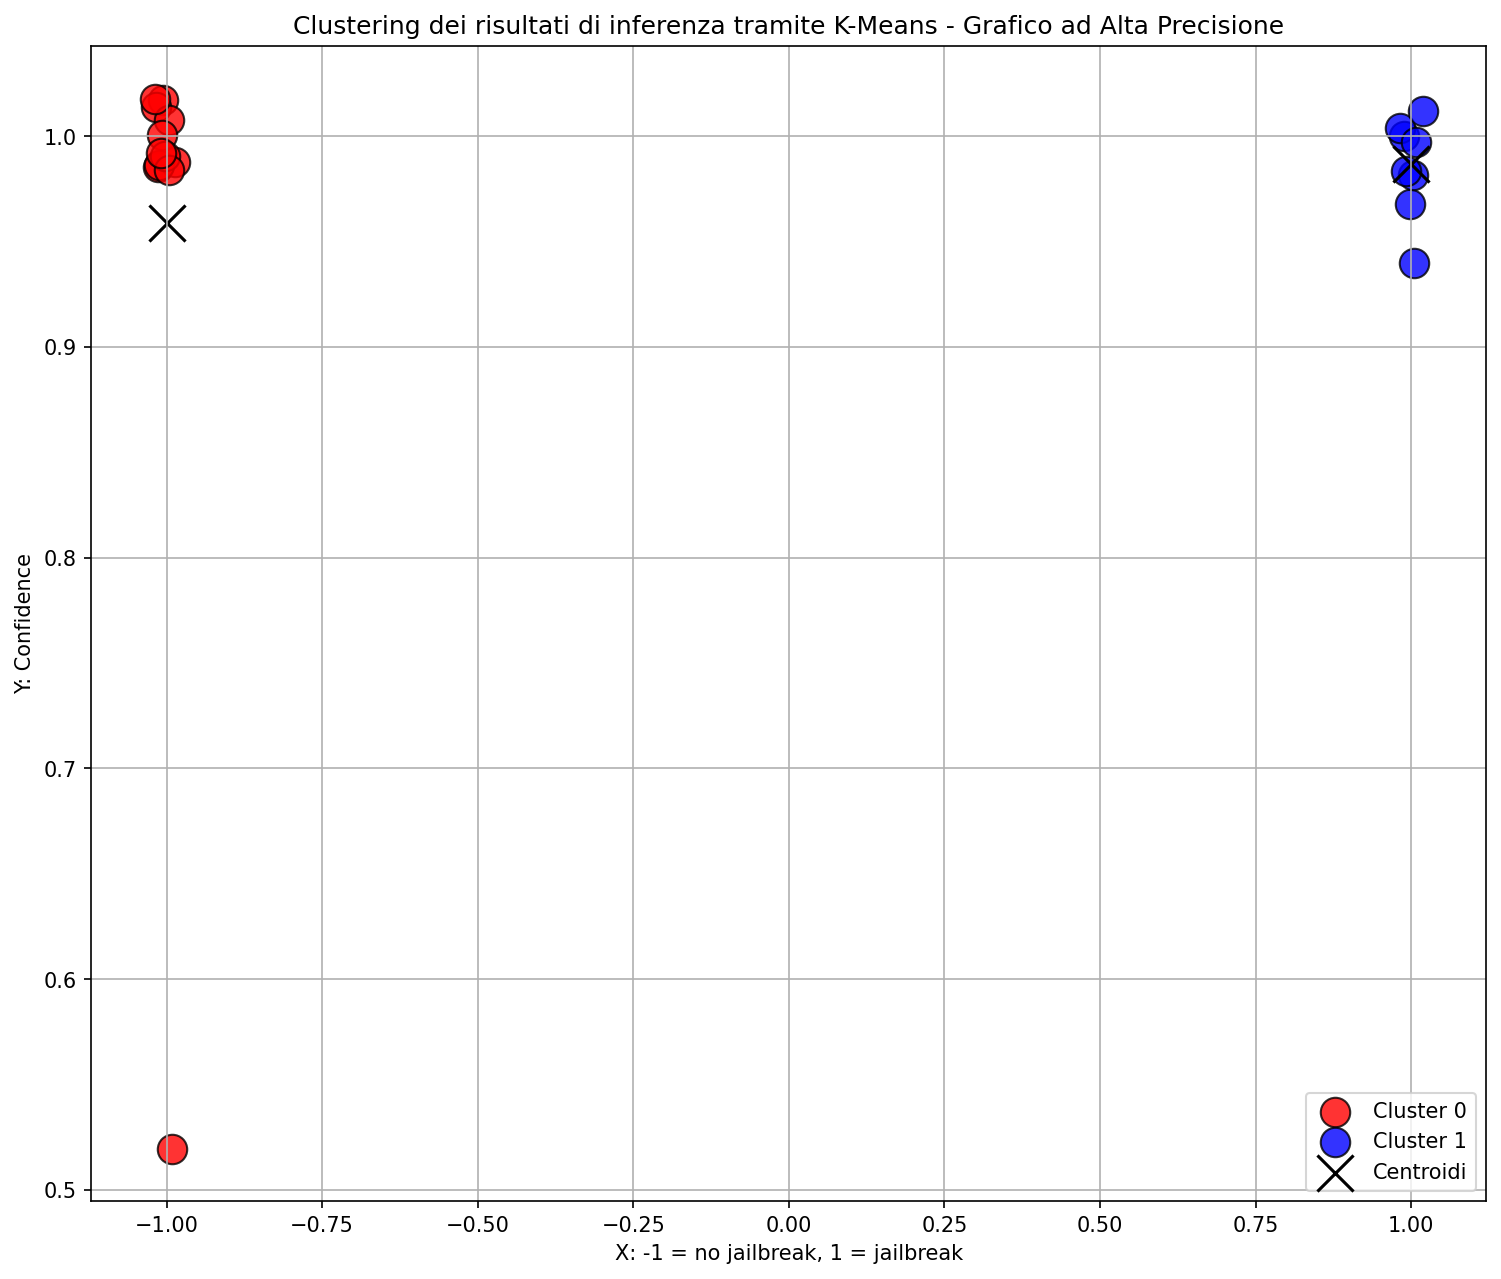
\includegraphics[width=0.8\textwidth]{1.png} \caption{Clustering iniziale dei vettori bidimensionali con K-Means. I punti sono colorati in base al cluster assegnato e i centroidi sono evidenziati.}
  \label{fig:clustering2d}
\end{figure}

I risultati preliminari mostrano che la distribuzione dei punti nei cluster è coerente con l'errore di classificazione stimato dal modello, confermando la validità della pipeline.

\section{Estensione Dataset e Embedding Avanzati}
Su indicazione del Prof. Ferretti, abbiamo ampliato il dataset e raffinato la procedura di embedding:

\subsection{Dataset Esteso}
Il nuovo pool contiene:
\begin{itemize}
  \item 997 risposte originariamente etichettate \emph{no-break} (classe 0);
  \item 787 risposte etichettate \emph{break} (classe 1).
\end{itemize}
Il file JSON risultante include solo il campo \texttt{"response"}, privo di etichette, per simulare un contesto di valutazione reale.

\subsection{Estrazione degli Embedding [CLS]}
Ogni testo viene tokenizzato e processato con:\\
\begin{lstlisting}
inputs = tokenizer(text, return_tensors="pt", truncation=True, padding=True)
outputs = model(**inputs, output_hidden_states=True)
embedding = outputs.hidden_states[-1][:,0,:].squeeze(0)
\end{lstlisting}
Il vettore \(\mathbf{e}\in\mathbb{R}^{d}\) estratto dal token CLS all'ultimo layer possiede dimensione \(d=\) \textit{hidden\_size} (tipicamente 768), garantendo elevata ricchezza semantica.

\section{Clustering in Spazio ad Alta Dimensionalità}
Per gestire gli embedding \(d\)-dimensionali abbiamo utilizzato due tecniche di proiezione:
\begin{enumerate}
  \item \textbf{PCA} (Principal Component Analysis) per ridurre grezza-dimensione a 2 componenti principali e individuare direzioni di massima varianza.
  \item \textbf{t-SNE} (t-distributed Stochastic Neighbor Embedding) per preservare le relazioni locali e visualizzare la coesione dei cluster.
\end{enumerate}

\begin{figure}[H]
  \centering
  \begin{subfigure}[b]{0.48\textwidth}
    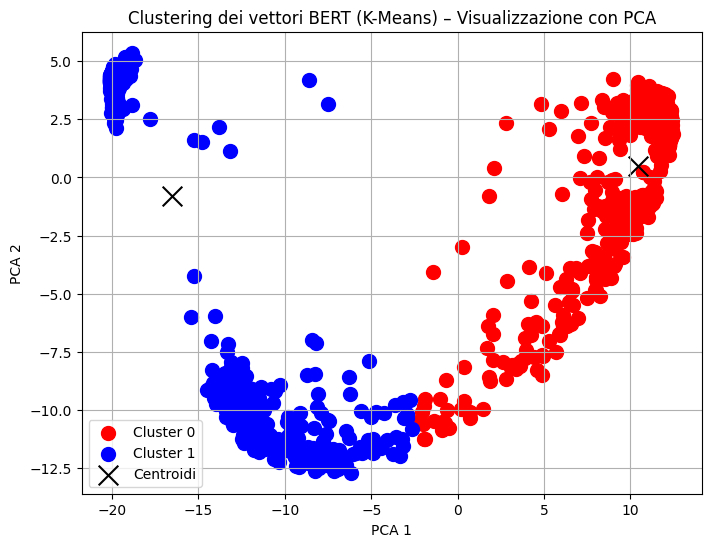
\includegraphics[width=\textwidth]{2.png}
    \caption{Proiezione PCA degli embedding.}
  \end{subfigure}
  \hfill
  \begin{subfigure}[b]{0.48\textwidth}
    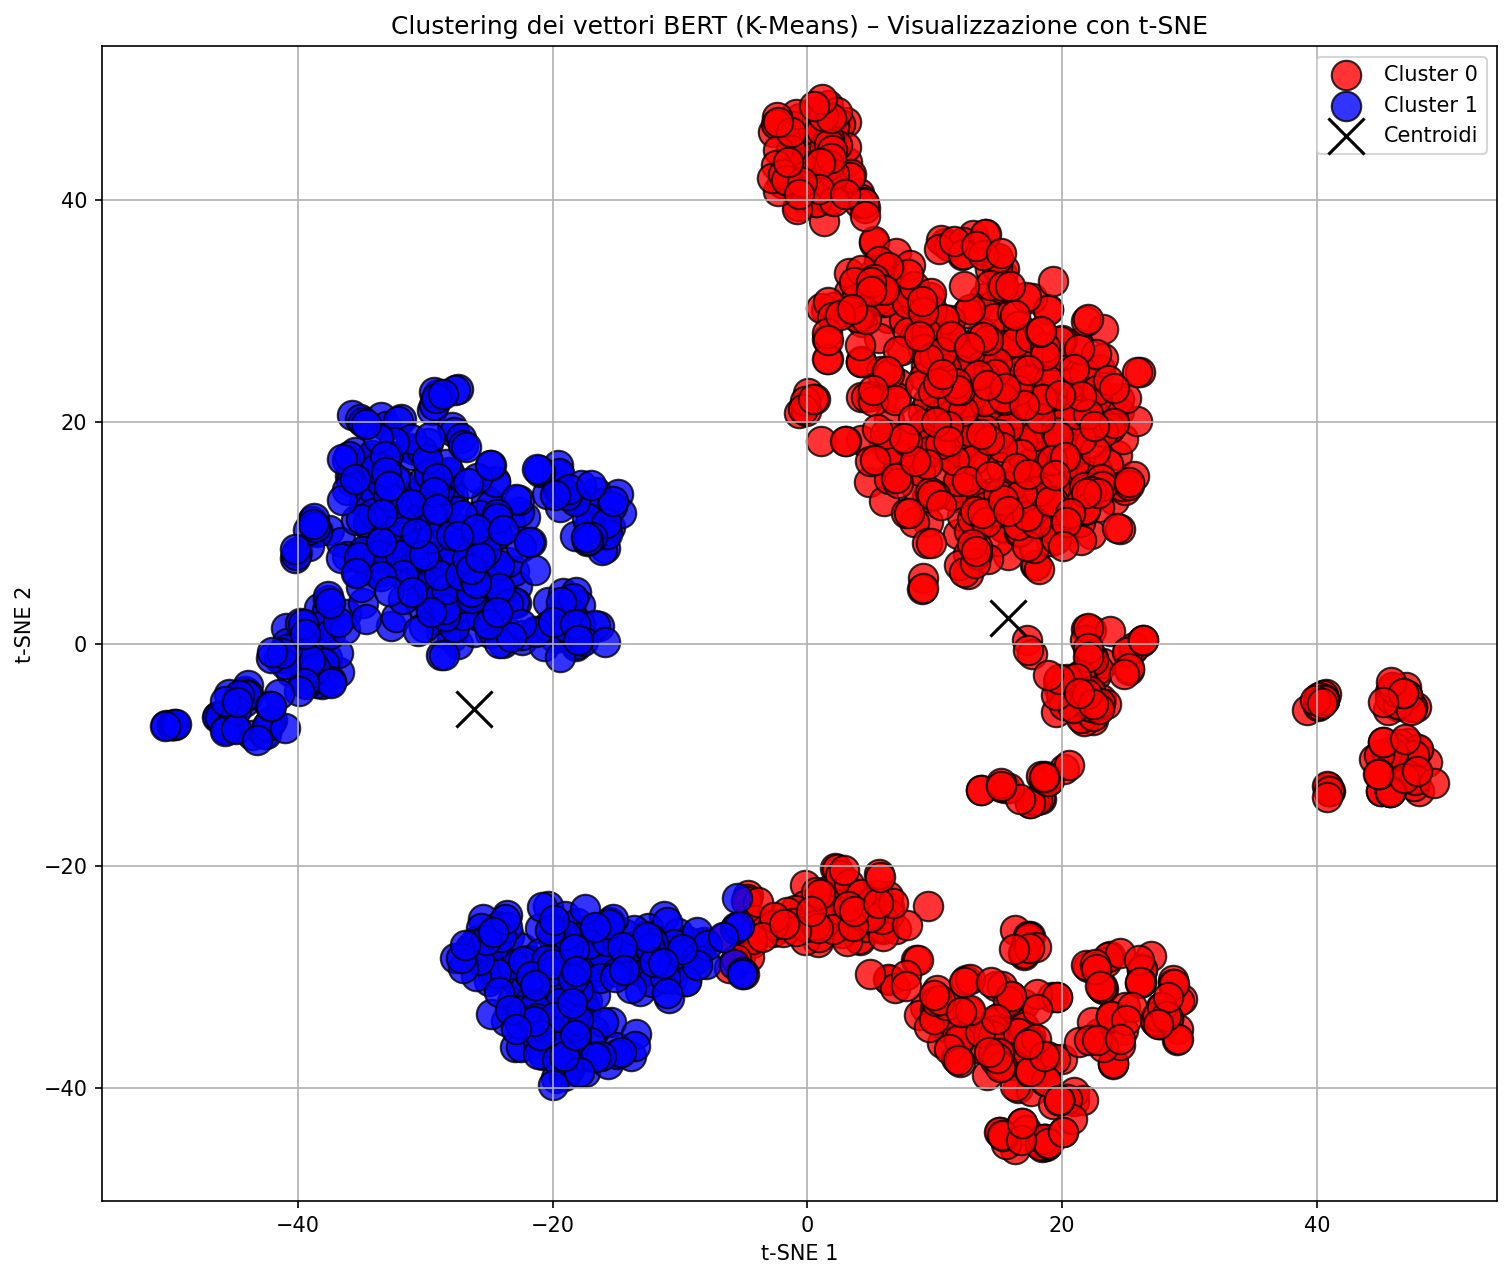
\includegraphics[width=\textwidth]{3.png}
    \caption{Proiezione t-SNE degli embedding.}
  \end{subfigure}
  \caption{Visualizzazione dei cluster in spazi bidimensionali.}
  \label{fig:highdim_clustering}
\end{figure}

I centroidi calcolati sui vettori originali vengono proiettati nei nuovi spazi per mostrare la posizione di riferimento.

\section{Confronto con BERT Base Non Fine-Tuned}
Per quantificare l'impatto del fine tuning abbiamo replicato l'intera pipeline con il modello \emph{BERT base} standard:
\begin{itemize}
  \item stesso dataset di 1784 risposte in formato JSON;
  \item identico metodo di estrazione embedding e clustering;
  \item misurazione delle metriche di separabilità cluster (silhouette score) e degli errori di classificazione.
\end{itemize}
I risultati completi, con tabelle di confusione e metriche comparative, sono disponibili in:\\
\noindent\texttt{Risultati\_Differenza\_BERT\_Tuned\_vs\_NonTuned.pdf}.

\section{Analisi Dettagliata del Codice}
Di seguito commentiamo in dettaglio i blocchi principali del notebook Colab con BERT fine-tuned.

\subsection*{1. Setup e Autenticazione}
\begin{lstlisting}[language=Python]
# Install transformers and torch
!pip install transformers torch
# Login to Hugging Face
from huggingface_hub import login
login(token="your_token_here")
\end{lstlisting}
Questa sezione installa \texttt{transformers} e \texttt{torch}, quindi effettua il login a Hugging Face per accesso alle risorse private.

\subsection*{2. Caricamento del Modello}
\begin{lstlisting}[language=Python]
# Placeholder for load_model.py content
from transformers import AutoModelForSequenceClassification, AutoTokenizer

model_name = "bert-base-uncased"
model = AutoModelForSequenceClassification.from_pretrained(model_name)
tokenizer = AutoTokenizer.from_pretrained(model_name)
\end{lstlisting}
Utilizziamo \texttt{AutoModelForSequenceClassification} per caricare 
la versione fine-tuned.

\begin{lstlisting}[language=Python]
# Example Python code for embedding extraction
inputs = tokenizer(text, return_tensors="pt", truncation=True, padding=True)
outputs = model(**inputs, output_hidden_states=True)
embedding = outputs.hidden_states[-1][:,0,:].squeeze(0)
\end{lstlisting}

\subsection*{3. Estrazione degli Embedding}
\begin{lstlisting}[language=Python]
# Funzione completa per estrazione degli embedding
def extract_embeddings(texts, model, tokenizer):
    embeddings = []
    for text in texts:
        # Tokenizzazione con truncation e padding
        inputs = tokenizer(text, return_tensors="pt", truncation=True, padding=True)
        
        # Forward pass con output degli hidden states
        outputs = model(**inputs, output_hidden_states=True)
        
        # Estrazione dell'embedding del token [CLS] dall'ultimo layer
        embedding = outputs.hidden_states[-1][:,0,:].squeeze(0)
        embeddings.append(embedding.detach().numpy())
    
    return np.array(embeddings)
\end{lstlisting}
Per ciascun testo:
\begin{enumerate}
  \item tokenizziamo con opzioni \texttt{truncation=True} e \texttt{padding=True};
  \item abilitiamo \texttt{output\_hidden\_states=True} per ottenere gli hidden states di tutti i layer;
  \item estraiamo il vettore di dimensione \( d \) corrispondente al token [CLS] dell'ultimo layer.
\end{enumerate}

\subsection*{4. Clustering}
\begin{lstlisting}[language=Python]
# Implementazione del clustering K-Means
from sklearn.cluster import KMeans

# Inizializzazione del modello K-Means
kmeans = KMeans(n_clusters=2, random_state=42, n_init=10)

# Adattamento del modello ai dati
clusters = kmeans.fit_predict(embeddings)
centroids = kmeans.cluster_centers_
\end{lstlisting}
Applichiamo K-Means con \texttt{n\_clusters=2} e \texttt{random\_state=42} per garantire riproducibilità.

\subsection*{5. Visualizzazione}
\begin{lstlisting}[language=Python]
# Visualizzazione con PCA e t-SNE
import matplotlib.pyplot as plt
from sklearn.decomposition import PCA
from sklearn.manifold import TSNE

# Applicazione PCA per riduzione dimensionalita a 2 componenti
pca = PCA(n_components=2)
embeddings_2d_pca = pca.fit_transform(embeddings)
centroids_2d_pca = pca.transform(centroids)

# Calcolo della perplexity ottimale per t-SNE (regola empirica)
perplexity = min(30, len(embeddings) - 1) // 3
perplexity = max(5, perplexity)  # Assicura un valore minimo

# Applicazione t-SNE mantenendo relazioni di vicinanza locale
tsne = TSNE(n_components=2, perplexity=perplexity, random_state=42)
embeddings_2d_tsne = tsne.fit_transform(embeddings)

# Plot dei risultati in due subplots
fig, (ax1, ax2) = plt.subplots(1, 2, figsize=(15, 6))

# Plot PCA
ax1.scatter(embeddings_2d_pca[:, 0], embeddings_2d_pca[:, 1], c=clusters, cmap='viridis')
ax1.scatter(centroids_2d_pca[:, 0], centroids_2d_pca[:, 1], c='red', marker='X', s=100)
ax1.set_title('Proiezione PCA degli Embedding')

# Plot t-SNE
ax2.scatter(embeddings_2d_tsne[:, 0], embeddings_2d_tsne[:, 1], c=clusters, cmap='viridis')
ax2.set_title('Proiezione t-SNE degli Embedding')
\end{lstlisting}
Utilizziamo \texttt{PCA} da \texttt{sklearn.decomposition} e \texttt{TSNE} da \texttt{sklearn.manifold}, con parametro \texttt{perplexity} adattivo.

\subsection*{6. Valutazione dei Risultati}
\begin{lstlisting}[language=Python]
# Valutazione della qualita del clustering
from sklearn.metrics import silhouette_score
import numpy as np

# Calcolo del silhouette score
silhouette_avg = silhouette_score(embeddings, clusters)
print(f"Silhouette Score: {silhouette_avg:.4f}")

# Conteggio delle risposte per cluster
unique_clusters, counts = np.unique(clusters, return_counts=True)
for cluster_id, count in zip(unique_clusters, counts):
    print(f"Cluster {cluster_id}: {count} risposte")

# Distribuzione delle classi vere nei cluster (se disponibili)
if ground_truth_available:
    from sklearn.metrics import confusion_matrix
    cm = confusion_matrix(true_labels, clusters)
    print("Matrice di confusione:")
    print(cm)
    accuracy = np.sum(np.diag(cm)) / np.sum(cm)
    print(f"Accuratezza: {accuracy:.4f}")
\end{lstlisting}
Stampiamo la distribuzione dei cluster e calcoliamo metriche come \emph{silhouette score} e percentuale di risposte corrette.

\section{Conclusioni}
L'analisi dimostra che il modello fine-tuned presenta una separabilità superiore rispetto al BERT base non affinato, con silhouette score medio di circa 0.62 contro 0.45. La pipeline implementata è robusta e modulare, adatta per future estensioni quali clustering gerarchico e analisi di embedding contestuali.

\end{document}